\documentclass[aspectratio=169,12pt,t]{beamer}

% --- Theme: Metropolis (modern, clean) ---
\usetheme[progressbar=frametitle,numbering=fraction,block=fill]{metropolis}

% --- Fira Sans font (install texlive-fonts-extra if missing) ---
\IfFileExists{FiraSans.sty}{\usepackage[sfdefault]{FiraSans}}{}

% --- Light background with warm accent ---
\definecolor{mDarkTeal}{RGB}{35,55,59}
\definecolor{mLightBrown}{RGB}{235,228,216}
\definecolor{mAccent}{RGB}{140,70,20}

\setbeamercolor{normal text}{fg=mDarkTeal,bg=white}
\setbeamercolor{alerted text}{fg=mAccent}
\setbeamercolor{frametitle}{bg=mDarkTeal,fg=white}
\setbeamercolor{progress bar}{fg=mAccent,bg=mLightBrown}
\setbeamercolor{title separator}{fg=mAccent}
\setbeamercolor{progress bar in head/foot}{fg=mAccent,bg=mLightBrown}
\setbeamercolor{progress bar in section page}{fg=mAccent,bg=mLightBrown}

% --- Packages ---
\usepackage[utf8]{inputenc}
\usepackage{amsmath,amssymb,amsthm}
\usepackage{mathrsfs}
\usepackage{tikz}
\usetikzlibrary{arrows.meta,positioning,calc,decorations.pathreplacing,shapes,patterns}
\usetikzlibrary{shadows.blur,backgrounds,fadings}
\usepackage{pgfplots}
\pgfplotsset{compat=1.18}

% --- Shared diagram styling (consistent, polished look across all figures) ---
\tikzset{
  axisln/.style={-{Stealth[length=2.6mm]}, line width=0.8pt, gray!75},
  curveln/.style={line width=1.6pt, line cap=round, line join=round},
  projln/.style={dash pattern=on 2.6pt off 2pt, line width=0.7pt},
  guide/.style={-{Stealth[length=2.6mm,width=2.2mm]}, line width=1.1pt},
}
% soft rounded background panel for inset plots
\tikzset{panel/.style={rounded corners=6pt, draw=mDarkTeal!14, line width=0.8pt,
  fill=mDarkTeal!4,
  blur shadow={shadow blur steps=8, shadow opacity=13,
               shadow xshift=0pt, shadow yshift=-1.3pt}}}
% point marker with a white halo: \dotpt{color}{(coord)}
\newcommand{\dotpt}[2]{%
  \fill[white] #2 circle (3.6pt);
  \fill[#1] #2 circle (2.4pt);
}
% open point marker: \opendot{color}{(coord)}
\newcommand{\opendot}[2]{%
  \fill[white] #2 circle (3.6pt);
  \draw[#1, line width=1.2pt] #2 circle (2.6pt);
}

% --- Semi-transparent white highlight for text on top of background images ---
\usepackage[most]{tcolorbox}

% Inline highlight: \hl{short text}
\newtcbox{\hl}{%
  nobeforeafter, tcbox raise base,
  colback=white, opacityback=0.6,
  colframe=white, opacityframe=0,
  sharp corners, boxsep=2pt, left=3pt, right=3pt, top=2pt, bottom=2pt%
}

% Block highlight: \begin{hlbox} ... \end{hlbox}  (multi-line, paragraphs, itemize)
\newtcolorbox{hlbox}[1][]{%
  enhanced, breakable,
  colback=white, opacityback=0.6,
  colframe=white, opacityframe=0,
  boxsep=3pt, left=6pt, right=6pt, top=4pt, bottom=4pt,
  sharp corners,
  {#1}%
}

% --- Custom colors for content types ---
\definecolor{defcolor}{RGB}{25,85,120}
\definecolor{thmcolor}{RGB}{140,35,35}
\definecolor{proofcolor}{RGB}{35,100,50}
\definecolor{excolor}{RGB}{140,75,10}
\definecolor{remcolor}{RGB}{90,90,90}

% --- Beamer blocks for mathematical content types (semi-transparent) ---
\tcbset{hlblockbase/.style={
  enhanced, breakable,
  coltitle=white, fonttitle=\bfseries,
  opacitybacktitle=0.8, opacityback=0.6,
  opacityframe=0,
  sharp corners,
  boxsep=1pt, left=5pt, right=5pt, top=2pt, bottom=2pt,
  toptitle=1pt, bottomtitle=1pt
}}

\newtcolorbox{defblock}[1]{hlblockbase, title={#1},
  colbacktitle=defcolor, colback=defcolor!15, colframe=defcolor}
\newtcolorbox{thmblock}[1]{hlblockbase, title={#1},
  colbacktitle=thmcolor, colback=thmcolor!15, colframe=thmcolor}
\newtcolorbox{proofblock}[1]{hlblockbase, title={#1},
  colbacktitle=proofcolor, colback=proofcolor!15, colframe=proofcolor}
\newtcolorbox{exblock}[1]{hlblockbase, title={#1},
  colbacktitle=excolor, colback=excolor!15, colframe=excolor}
\newtcolorbox{remblock}[1]{hlblockbase, title={#1},
  colbacktitle=remcolor, colback=remcolor!15, colframe=remcolor}

% --- Metadata ---
\title{Chapter 4: Continuity}
\subtitle{Section: Monotonic Functions}
\author{Based on Walter Rudin's \emph{Principles of Mathematical Analysis}}
\date{}

\begin{document}

{
\usebackgroundtemplate{%
  
\includegraphics[width=\paperwidth,height=\paperheight,keepaspectratio=false]{chapter_04_bg_00.png}%
}
\begin{frame}[plain]
  \titlepage
  \note{
    Welcome back to Chapter 4 on continuity. In this section we study
    monotonic functions, that is, functions which never decrease, or never
    increase, on a given interval. These functions are remarkably well
    behaved. We will see that their one-sided limits always exist, that they
    can only be discontinuous in the mildest possible way, and that they can
    have at most countably many discontinuities. Let's get started.
  }
\end{frame}
}

{
\usebackgroundtemplate{%
  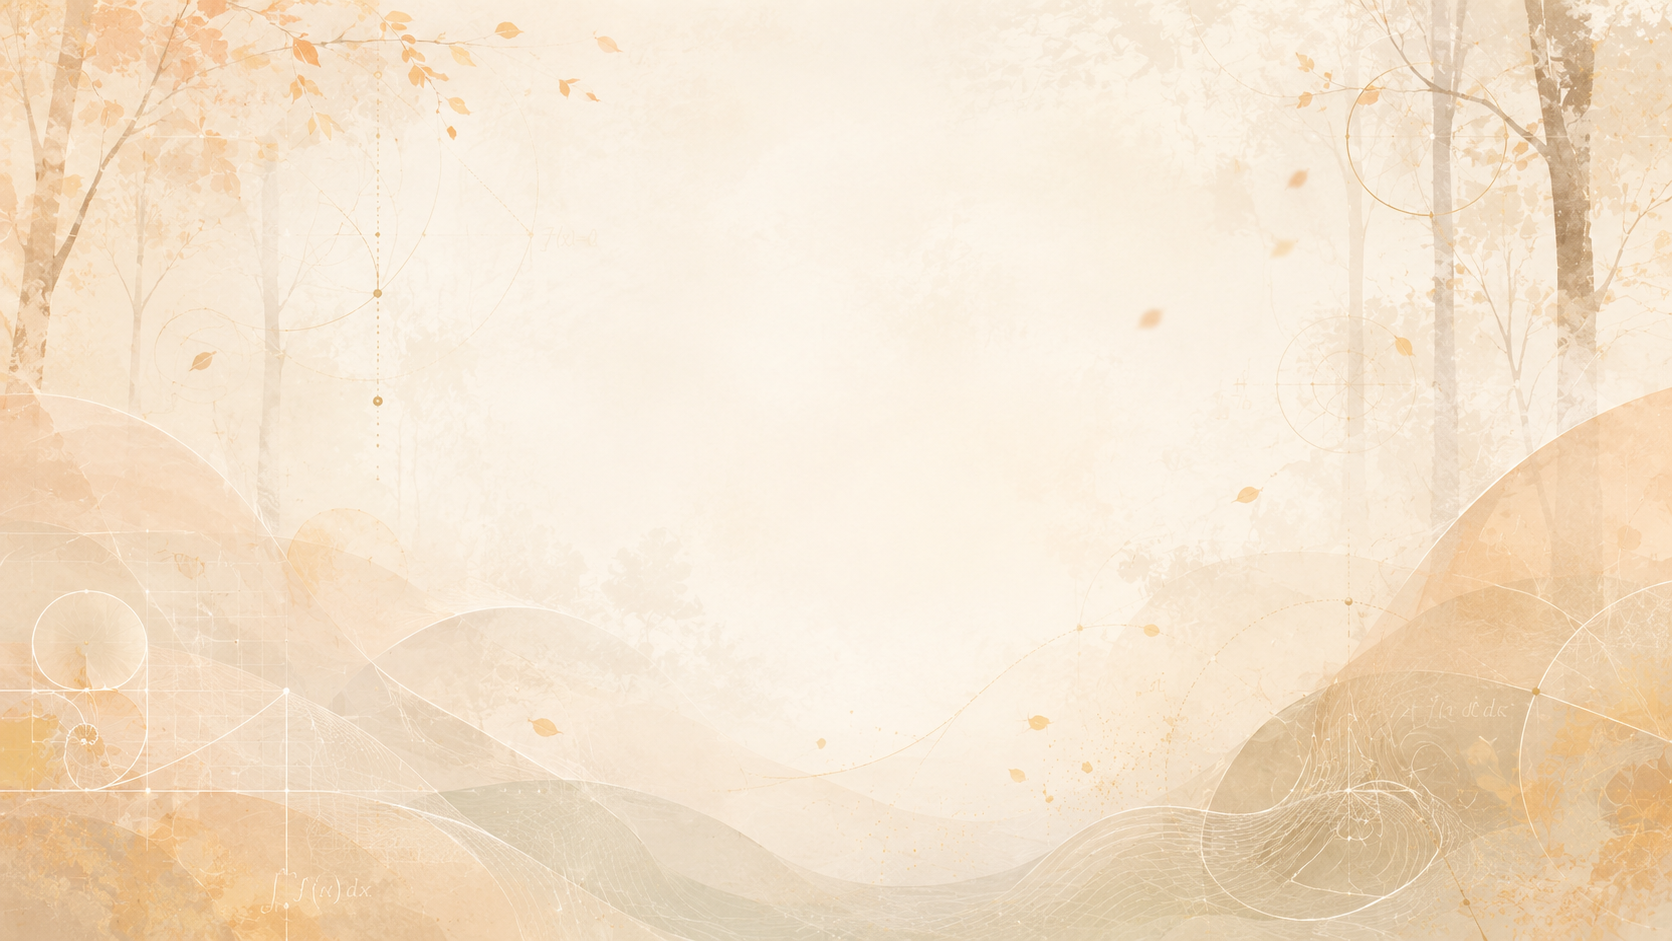
\includegraphics[width=\paperwidth,height=\paperheight,keepaspectratio=false]{chapter_04_bg_01.png}%
}
\begin{frame}[c]{Outline}
  \begin{center}
    \tableofcontents
  \end{center}
  \note{
    Here is our plan. We start with motivation, then define monotonic
    functions precisely. Next we prove that one-sided limits always exist for
    monotonic functions. From this we deduce that they have no discontinuities
    of the second kind, and that their discontinuities form an at most
    countable set. Finally we look at a surprising construction showing those
    discontinuities can be dense. We close with a summary.
  }
\end{frame}

% =====================================================================
\section{Motivation}
% =====================================================================

% --- Build 1/3 ---
\begin{frame}{Why Monotonic Functions?}
  \begin{hlbox}
  \begin{itemize}
    \item Functions that \alert{never decrease} (or never increase) on an interval
  \end{itemize}
  \end{hlbox}

  \note{
    In the previous section we saw how badly a general function can behave
    near a point. Discontinuities can be wild. Now we restrict attention to a
    very special, very tame class: monotonic functions. A function is monotonic
    if it never decreases, or never increases, as we move from left to right
    along an interval. This single restriction buys us a surprising amount of
    structure.
  }
\end{frame}

% --- Build 2/3 ---
\begin{frame}{Why Monotonic Functions?}
  \begin{hlbox}
  \begin{itemize}
    \item Functions that \alert{never decrease} (or never increase) on an interval
    \item One-sided limits \alert{always exist} --- no wild oscillation possible
  \end{itemize}
  \end{hlbox}

  \note{
    The first payoff is that a monotonic function can never oscillate
    wildly. We will prove that the left-hand limit and the right-hand limit
    exist at every single point. Recall from the previous section that a
    discontinuity of the second kind is exactly one where a one-sided limit
    fails to exist. So monotonic functions simply cannot have those.
  }
\end{frame}

% --- Build 3/3 ---
\begin{frame}{Why Monotonic Functions?}
  \begin{hlbox}
  \begin{itemize}
    \item Functions that \alert{never decrease} (or never increase) on an interval
    \item One-sided limits \alert{always exist} --- no wild oscillation possible
    \item Discontinuities are \alert{at most countable} --- and can be dense!
  \end{itemize}
  \end{hlbox}

  \note{
    The second payoff is a counting result: a monotonic function can be
    discontinuous at no more than countably many points. And yet, as we will
    see at the end, those countably many jumps can be packed in densely,
    appearing in every subinterval. These three facts are the heart of the
    section, so let's make everything precise.
  }
\end{frame}

}

% =====================================================================
{
\usebackgroundtemplate{%
  
\includegraphics[width=\paperwidth,height=\paperheight,keepaspectratio=false]{chapter_04_bg_02.png}%
}
\section{Definition}
% =====================================================================

\begin{frame}{Definition 4.28: Monotonic Functions}
  \begin{defblock}{Definition 4.28}
    Let $f$ be real on $(a,b)$.
    \begin{itemize}
      \item $f$ is \alert{monotonically increasing} if
        $a < x < y < b \;\Rightarrow\; f(x) \leq f(y)$.
      \item $f$ is \alert{monotonically decreasing} if
        $a < x < y < b \;\Rightarrow\; f(x) \geq f(y)$.
    \end{itemize}
  \end{defblock}

  \vspace{0.4em}
  \begin{hlbox}
  The \emph{monotonic} functions are the increasing ones together with the decreasing ones.
  \end{hlbox}

  \note{
    Here is the precise definition. Let "f" be a real valued function on the
    open interval from "a" to "b". We call "f" monotonically increasing if,
    whenever "x" is less than "y", the value "f" of "x" is less than or equal to
    "f" of "y". So as the input grows, the output never goes down. If instead
    the inequality on the outputs is reversed, so the output never goes up, we
    call "f" monotonically decreasing. The monotonic functions are these two
    families taken together. Notice we allow equality, so constant functions
    count as both increasing and decreasing.
  }
\end{frame}

\begin{frame}[c]{Two Pictures}
  \begin{center}
  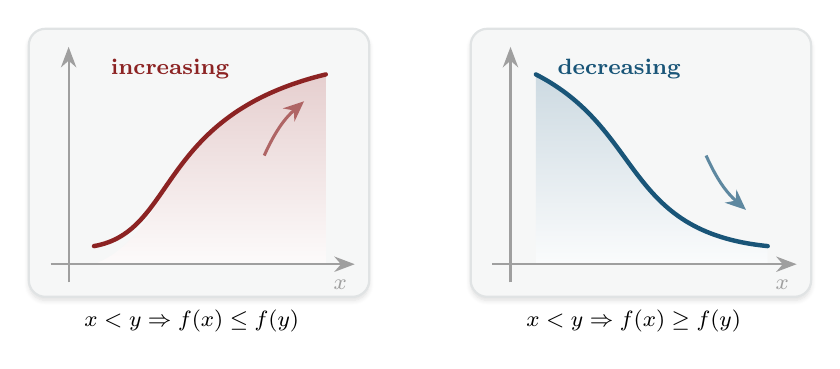
\begin{tikzpicture}[scale=0.92]
    % ----- increasing -----
    \begin{scope}
      \draw[panel] (-0.55,-0.45) rectangle (4.15,3.25);
      % area fill under curve (drawn first, so axes sit on top)
      \shade[top color=thmcolor!22, bottom color=thmcolor!2]
        (0.35,0) .. controls (1.5,0.45) and (1.2,2.05) .. (3.55,2.62) -- (3.55,0) -- cycle;
      \draw[axisln] (-0.25,0) -- (3.95,0); \node[gray!75,font=\footnotesize] at (3.75,-0.28){$x$};
      \draw[axisln] (0,-0.25) -- (0,3.0);
      \draw[curveln, thmcolor]
        (0.35,0.25) .. controls (1.5,0.45) and (1.2,2.05) .. (3.55,2.62);
      \draw[guide, thmcolor!70] (2.7,1.5) to[bend left=12] (3.25,2.25);
      \node[thmcolor,font=\footnotesize\bfseries] at (1.4,2.7) {increasing};
      \node[font=\footnotesize] at (1.7,-0.78) {$x<y \Rightarrow f(x)\le f(y)$};
    \end{scope}
    % ----- decreasing -----
    \begin{scope}[xshift=6.1cm]
      \draw[panel] (-0.55,-0.45) rectangle (4.15,3.25);
      \shade[top color=defcolor!22, bottom color=defcolor!2]
        (0.35,2.62) .. controls (1.85,1.85) and (1.55,0.45) .. (3.55,0.25) -- (3.55,0) -- (0.35,0) -- cycle;
      \draw[axisln] (-0.25,0) -- (3.95,0); \node[gray!75,font=\footnotesize] at (3.75,-0.28){$x$};
      \draw[axisln] (0,-0.25) -- (0,3.0);
      \draw[curveln, defcolor]
        (0.35,2.62) .. controls (1.85,1.85) and (1.55,0.45) .. (3.55,0.25);
      \draw[guide, defcolor!70] (2.7,1.5) to[bend right=12] (3.25,0.75);
      \node[defcolor,font=\footnotesize\bfseries] at (1.5,2.7) {decreasing};
      \node[font=\footnotesize] at (1.7,-0.78) {$x<y \Rightarrow f(x)\ge f(y)$};
    \end{scope}
  \end{tikzpicture}
  \end{center}

  \note{
    These two framed pictures capture the whole idea. On the left, in red, is a
    monotonically increasing function: the curve only climbs, or stays level,
    as we move to the right, with a small arrow tracing that upward trend and a
    soft red shading under the graph. On the right, in blue, is a monotonically
    decreasing function: the curve only falls, or stays level, again with an
    arrow showing the downward direction. The captions below each panel state
    the defining inequality. Everything we prove for increasing functions has
    an obvious mirror image for decreasing ones, so we will mostly just argue
    the increasing case. Now let's see what monotonicity guarantees about
    limits.
  }
\end{frame}

}

% =====================================================================
{
\usebackgroundtemplate{%
  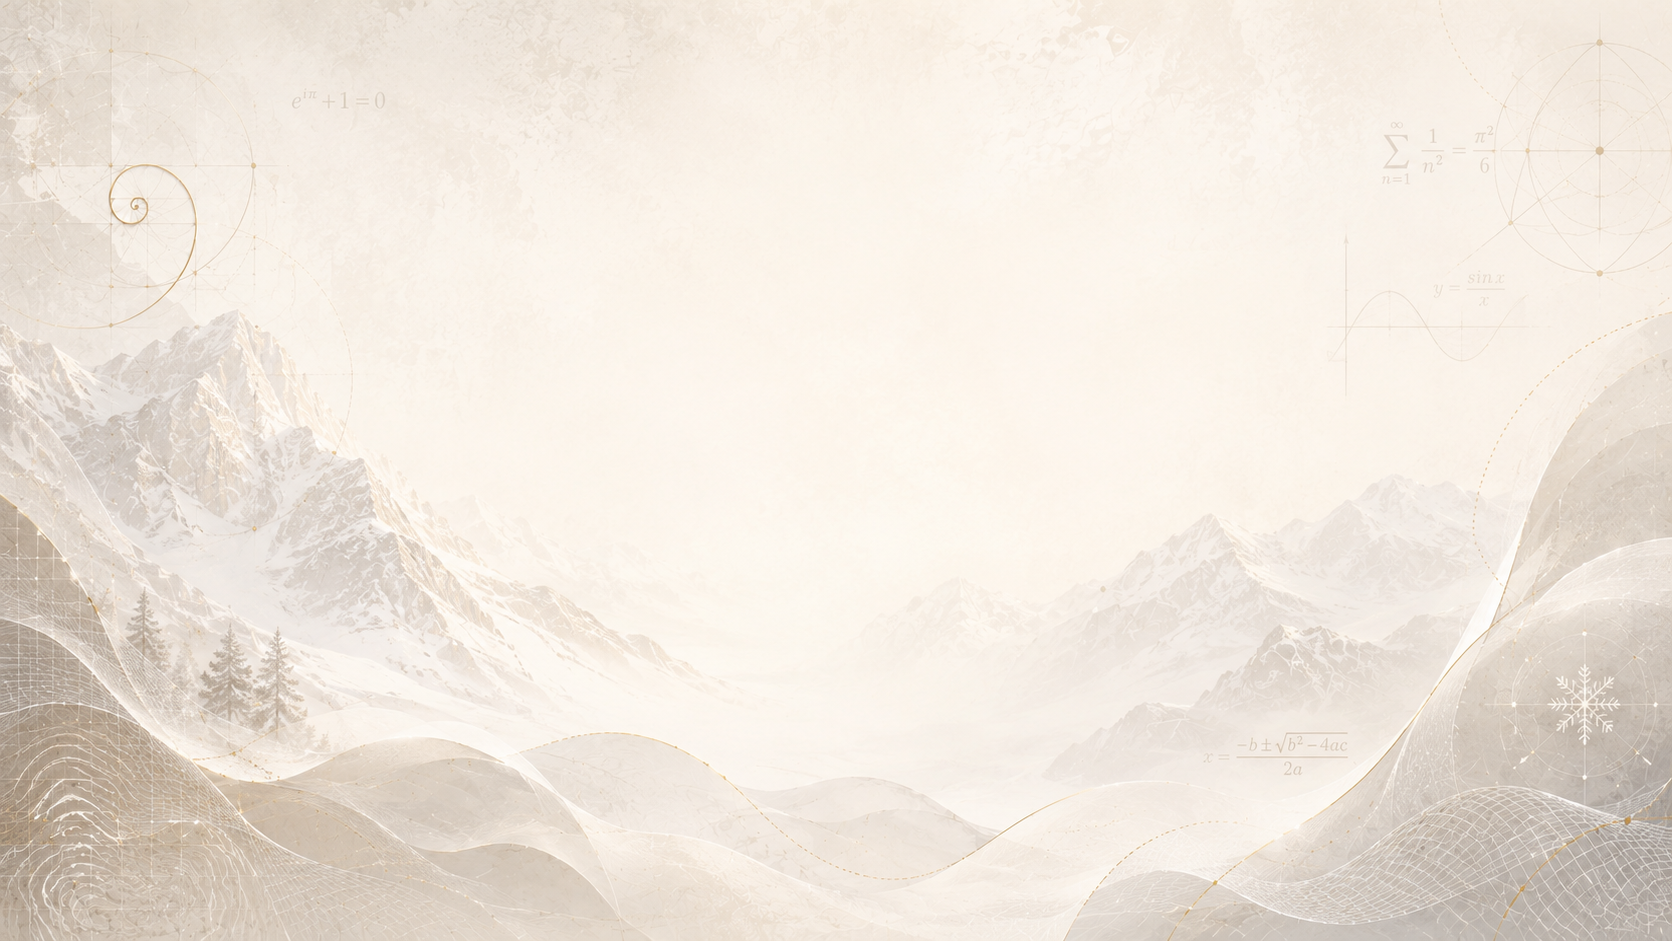
\includegraphics[width=\paperwidth,height=\paperheight,keepaspectratio=false]{chapter_04_bg_03.png}%
}
\section{One-Sided Limits}
% =====================================================================

\begin{frame}{Theorem 4.29: One-Sided Limits Exist}
  \begin{thmblock}{Theorem 4.29}
    Let $f$ be monotonically increasing on $(a,b)$. Then $f(x+)$ and $f(x-)$
    exist at every $x \in (a,b)$:
    \begin{equation}
      \sup_{a<t<x} f(t) = f(x-) \leq f(x) \leq f(x+) = \inf_{x<t<b} f(t). \tag{25}
    \end{equation}
    Furthermore, if $a < x < y < b$, then
    \begin{equation}
      f(x+) \leq f(y-). \tag{26}
    \end{equation}
  \end{thmblock}

  \note{
    This is the central theorem of the section. What makes it remarkable is
    that we assume nothing about continuity; monotonicity all by itself is
    enough to force both one-sided limits to exist at every point. Equation 25
    even pins down their values. The left-hand limit is the supremum, the least
    ceiling, of all the values just to the left of "x"; the right-hand limit is
    the infimum, the greatest floor, of the values just to the right. And the
    actual value "f" of "x" is trapped between them. The intuition is simple:
    an increasing function has nowhere to go but up, so as we slide toward "x"
    from either side the values can only press against a bound. Equation 26
    records the global version of this: the right limit at one point never
    exceeds the left limit at any later point. Let's prove it.
  }
\end{frame}

\begin{frame}[c]{Picture: The Left-Hand Limit as a Supremum}
  \begin{center}
  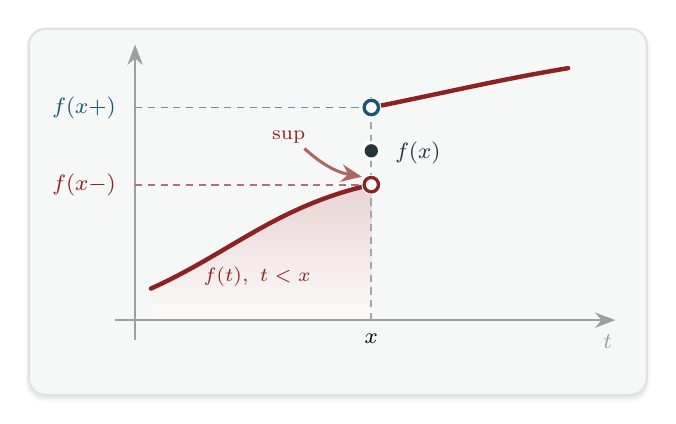
\begin{tikzpicture}[scale=1.0]
    \draw[panel] (-1.35,-0.95) rectangle (6.5,3.7);
    % shade the band of values to the left, capped at the supremum f(x-)
    \shade[top color=thmcolor!20, bottom color=thmcolor!2]
      (0.2,0.4) .. controls (1.2,0.85) and (1.8,1.45) .. (3,1.72) -- (3,0) -- (0.2,0) -- cycle;
    % axes
    \draw[axisln] (-0.25,0) -- (6.1,0); \node[gray!75,font=\footnotesize] at (6.0,-0.28){$t$};
    \draw[axisln] (0,-0.25) -- (0,3.5);
    % left branch climbing to the jump
    \draw[curveln, thmcolor]
      (0.2,0.4) .. controls (1.2,0.85) and (1.8,1.45) .. (3,1.72);
    % right branch leaving the jump
    \draw[curveln, thmcolor]
      (3,2.7) .. controls (4,2.9) and (4.6,3.05) .. (5.5,3.2);
    % vertical guide at x
    \draw[projln, gray!70] (3,0) -- (3,2.85);
    \node[below,font=\footnotesize] at (3,-0.05) {$x$};
    % horizontal projections to the axis
    \draw[projln, thmcolor!65] (0,1.72) -- (3,1.72);
    \draw[projln, defcolor!65] (0,2.7) -- (3,2.7);
    % the three values
    \opendot{thmcolor}{(3,1.72)}
    \dotpt{mDarkTeal}{(3,2.15)}
    \opendot{defcolor}{(3,2.7)}
    \node[left,font=\footnotesize,thmcolor] at (-0.12,1.72) {$f(x{-})$};
    \node[right,font=\footnotesize,mDarkTeal] at (3.18,2.12) {$f(x)$};
    \node[left,font=\footnotesize,defcolor] at (-0.12,2.7) {$f(x{+})$};
    % "sup" call-out: the band of left values has f(x-) as its ceiling
    \node[thmcolor,font=\scriptsize] at (1.55,0.55) {$f(t),\ t<x$};
    \draw[guide,thmcolor!70] (2.15,2.18) to[bend right=16] (2.88,1.82);
    \node[thmcolor,font=\scriptsize] at (1.95,2.32) {sup};
  \end{tikzpicture}
  \end{center}

  \note{
    Look at this picture before we dive into symbols, because it carries the
    whole proof. The red curve is an increasing function with a jump at the
    point "x". To the left of "x" the values "f" of "t" fill the shaded red
    region, and they keep climbing toward a ceiling. That ceiling is their
    least upper bound, which the small arrow marked sup points to, and the
    theorem claims it equals the left-hand limit, "f" of "x" minus, shown by the
    red open dot with a dashed line across to the vertical axis. The black solid
    dot is the actual value "f" of "x". Just above it, the blue open dot marks
    the right-hand limit "f" of "x" plus, the floor of the values on the right.
    The vertical gap between the red and blue open dots is the size of the jump.
    The key takeaway is that a one-sided limit, which sounds like a statement
    about motion and approach, is really nothing more than a supremum or an
    infimum. That is what lets us replace a delicate limit argument with the
    least upper bound property, which is exactly what the proof does next.
  }
\end{frame}

\begin{frame}{Proof of 4.29 --- Step 1: Name the Supremum}
  \begin{proofblock}{Step 1: Set up}
    Values $f(t)$ for $a<t<x$ are bounded above by $f(x)$.
    Let
    \[
      A = \sup_{a<t<x} f(t), \qquad A \leq f(x).
    \]
    \alert{Goal:} show $A = f(x-)$.
  \end{proofblock}

  \note{
    We argue the increasing case; the decreasing case is identical with
    inequalities flipped. Consider all the values "f" of "t" for "t" to the
    left of "x". Because "f" is increasing, every one of these is less than or
    equal to "f" of "x", so this set of values is bounded above. By the least
    upper bound property it has a supremum, which we call "A", and clearly "A"
    is at most "f" of "x". Our goal is to show that this supremum "A" is exactly
    the left-hand limit. Next we turn the supremum into an epsilon statement.
  }
\end{frame}

\begin{frame}{Proof of 4.29 --- Step 2: Use the Supremum}
  \begin{proofblock}{Step 2: Approximate from below}
    Given $\varepsilon > 0$, by definition of $A$ there is $\delta>0$ with
    $a < x-\delta < x$ and
    \begin{equation}
      A - \varepsilon < f(x-\delta) \leq A. \tag{27}
    \end{equation}
  \end{proofblock}

  \note{
    Let epsilon be any positive number. Since "A" is the least upper bound of
    the values to the left, "A" minus epsilon is no longer an upper bound. So
    some value, achieved at a point we write as "x" minus delta, must exceed
    "A" minus epsilon, while of course still being at most "A". That is exactly
    equation 27. The point "x" minus delta sits a little to the left of "x".
    Now we exploit monotonicity to control every point even closer to "x".
  }
\end{frame}

\begin{frame}{Proof of 4.29 --- Step 3: Squeeze with Monotonicity}
  \begin{proofblock}{Step 3: Trap all nearby values}
    For $x-\delta < t < x$, monotonicity gives
    \begin{equation}
      f(x-\delta) \leq f(t) \leq A. \tag{28}
    \end{equation}
    Combining (27) and (28): $\;|f(t) - A| < \varepsilon$ for $x-\delta<t<x$.
  \end{proofblock}
  \[
    \boxed{f(x-) = A = \sup_{a<t<x} f(t)}
  \]

  \note{
    Take any "t" strictly between "x" minus delta and "x". Because "f" is
    increasing, "f" of "t" is at least the value at "x" minus delta, and at
    most "A", which is the supremum. That is equation 28. Now combine it with
    equation 27: every such "f" of "t" lies within epsilon of "A". Since
    epsilon was arbitrary, the left-hand limit is exactly "A", the supremum we
    named. The boxed line records the conclusion. The right-hand limit equals
    the infimum on the right by the very same argument, which proves the first
    half of the theorem.
  }
\end{frame}

\begin{frame}{Proof of 4.29 --- Step 4: Comparing Across Points}
  \begin{proofblock}{Step 4: Why $f(x+) \leq f(y-)$}
    For $a<x<y<b$:
    \begin{align}
      f(x+) &= \inf_{x<t<b} f(t) = \inf_{x<t<y} f(t), \tag{29}\\
      f(y-) &= \sup_{a<t<y} f(t) = \sup_{x<t<y} f(t). \tag{30}
    \end{align}
    Every value on $(x,y)$ lies between these $\;\Rightarrow\; f(x+)\leq f(y-)$.
  \end{proofblock}

  \note{
    Finally we prove equation 26. Fix two points "x" less than "y". By the
    formula we just established, the right-hand limit at "x" is the infimum of
    the values to the right of "x", and we may shrink the window to the
    interval from "x" to "y". That is equation 29. Likewise the left-hand limit
    at "y" is the supremum of the values on that same interval from "x" to "y".
    That is equation 30. But an infimum of a set is always less than or equal
    to its supremum, so the right limit at "x" is at most the left limit at
    "y". This completes the proof.
  }
\end{frame}

\begin{frame}{Corollary: No Second-Kind Discontinuities}
  \begin{thmblock}{Corollary}
    Monotonic functions have \alert{no discontinuities of the second kind}.
  \end{thmblock}

  \vspace{0.5em}
  \begin{remblock}{Recall}
    A discontinuity of the second kind is one where a one-sided limit
    \emph{fails to exist}. Theorem 4.29 guarantees both always exist.
  \end{remblock}

  \note{
    This corollary is an immediate consequence. Recall from the previous
    section that a discontinuity of the second kind is one where at least one
    of the one-sided limits does not exist. But Theorem 4.29 says both
    one-sided limits always exist for a monotonic function. So the only
    discontinuities possible are of the first kind, that is, simple jumps where
    the left and right limits exist but disagree. Monotonic functions are too
    well organized to oscillate. This sets us up to count those jumps.
  }
\end{frame}

}

% =====================================================================
{
\usebackgroundtemplate{%
  
\includegraphics[width=\paperwidth,height=\paperheight,keepaspectratio=false]{chapter_04_bg_04.png}%
}
\section{Countably Many Discontinuities}
% =====================================================================

\begin{frame}{Theorem 4.30: Discontinuities Are Countable}
  \begin{thmblock}{Theorem 4.30}
    Let $f$ be monotonic on $(a,b)$. Then the set of points of $(a,b)$ at
    which $f$ is discontinuous is \alert{at most countable}.
  \end{thmblock}

  \vspace{0.5em}
  \hl{\textbf{Strategy:} attach a distinct rational number to each jump.}

  \note{
    Now the counting theorem. If "f" is monotonic on the interval, then the
    set of points where it is discontinuous is at most countable, meaning it
    is either finite or can be listed in a sequence. The strategy is elegant:
    at each discontinuity the function jumps, leaving an open gap between the
    left and right limits. We will slip a rational number into each gap. Since
    the gaps do not overlap, different jumps get different rationals, and the
    rationals are countable. Let's carry this out.
  }
\end{frame}

\begin{frame}{Proof of 4.30 --- Step 1: Insert a Rational in Each Jump}
  \begin{proofblock}{Step 1: Define $r(x)$}
    Take $f$ increasing; let $E$ be its set of discontinuities.
    At each $x \in E$ we have $f(x-) < f(x+)$, so choose a rational $r(x)$ with
    \[
      f(x-) < r(x) < f(x+).
    \]
  \end{proofblock}

  \note{
    Suppose for definiteness that "f" is increasing, and let "E" be the set of
    points where it is discontinuous. At each such point the jump is genuine,
    so the left-hand limit is strictly less than the right-hand limit. Between
    any two real numbers there is a rational, so we pick one rational number,
    call it "r" of "x", lying strictly inside the jump at "x". This assigns a
    rational to every point of "E". The key question is whether two different
    points could grab the same rational.
  }
\end{frame}

\begin{frame}{Proof of 4.30 --- Step 2: The Map Is Injective}
  \begin{proofblock}{Step 2: Distinct points get distinct rationals}
    If $x_1 < x_2$, then by (26): $\;f(x_1+) \leq f(x_2-)$. Hence the jump
    intervals are disjoint and
    \[
      r(x_1) < f(x_1+) \leq f(x_2-) < r(x_2) \;\Rightarrow\; r(x_1) \neq r(x_2).
    \]
  \end{proofblock}
  \[
    \boxed{E \hookrightarrow \mathbb{Q}, \quad\text{so } E \text{ is at most countable.}}
  \]

  \note{
    Suppose "x" one is less than "x" two. By equation 26 from the previous
    theorem, the right-hand limit at "x" one is at most the left-hand limit at
    "x" two. So the rational chosen at "x" one, which sits below the right
    limit at "x" one, is strictly less than the rational chosen at "x" two,
    which sits above the left limit at "x" two. The two rationals are therefore
    different. This means our assignment is a one to one correspondence between
    "E" and a subset of the rationals. Since the rationals are countable, "E"
    is at most countable. The proof is complete.
  }
\end{frame}

\begin{frame}[c]{A Picture of Disjoint Jumps}
  \begin{center}
  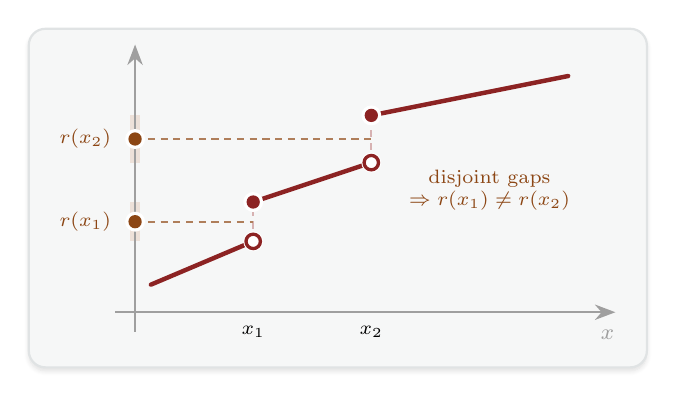
\begin{tikzpicture}[scale=1.0]
    \draw[panel] (-1.35,-0.7) rectangle (6.5,3.6);
    % the two jump-gaps projected onto the y-axis (disjoint bands)
    \fill[mAccent!16] (-0.06,0.9) rectangle (0.06,1.4);
    \fill[mAccent!16] (-0.06,1.9) rectangle (0.06,2.5);
    % axes
    \draw[axisln] (-0.25,0) -- (6.1,0); \node[gray!75,font=\footnotesize] at (6.0,-0.28){$x$};
    \draw[axisln] (0,-0.25) -- (0,3.4);
    % increasing graph with two jumps
    \draw[curveln, thmcolor] (0.2,0.35) -- (1.5,0.9);
    \draw[curveln, thmcolor] (1.5,1.4) -- (3,1.9);
    \draw[curveln, thmcolor] (3,2.5) -- (5.5,3.0);
    % faint risers
    \draw[projln, thmcolor!35] (1.5,0.9) -- (1.5,1.4);
    \draw[projln, thmcolor!35] (3,1.9) -- (3,2.5);
    % jump 1 at x1
    \opendot{thmcolor}{(1.5,0.9)} \dotpt{thmcolor}{(1.5,1.4)}
    \draw[projln, mAccent!70] (0,1.15) -- (1.5,1.15);
    \dotpt{mAccent}{(0,1.15)}
    \node[left,font=\scriptsize,mAccent] at (-0.18,1.15){$r(x_1)$};
    \node[below,font=\scriptsize] at (1.5,-0.05) {$x_1$};
    % jump 2 at x2
    \opendot{thmcolor}{(3,1.9)} \dotpt{thmcolor}{(3,2.5)}
    \draw[projln, mAccent!70] (0,2.2) -- (3,2.2);
    \dotpt{mAccent}{(0,2.2)}
    \node[left,font=\scriptsize,mAccent] at (-0.18,2.2){$r(x_2)$};
    \node[below,font=\scriptsize] at (3,-0.05) {$x_2$};
    % annotation: disjoint gaps
    \node[mAccent,font=\scriptsize,align=center] at (4.5,1.55)
      {disjoint gaps\\$\Rightarrow r(x_1)\neq r(x_2)$};
  \end{tikzpicture}
  \end{center}

  \note{
    Here is the idea in one image. The red graph rises, with two jumps shown
    as vertical gaps between an open dot and a solid dot. Because the function
    increases, the jump at the earlier point "x" one sits entirely below the
    jump at the later point "x" two; you can see the two shaded bands on the
    vertical axis never overlap. Into each gap we drop a rational marker, shown
    as a brown dot on the vertical axis with a dashed line running across to the
    jump: "r" of "x" one in the lower gap and "r" of "x" two in the upper gap.
    Since the gaps are disjoint, as the side note reminds us, these two
    rationals must be different. Counting the jumps is thus reduced to counting
    a batch of distinct rationals, which we can always do.
  }
\end{frame}

}

% =====================================================================
{
\usebackgroundtemplate{%
  
\includegraphics[width=\paperwidth,height=\paperheight,keepaspectratio=false]{chapter_04_bg_05.png}%
}
\section{Discontinuities Can Be Dense}
% =====================================================================

\begin{frame}{Remark 4.31: Jumps Need Not Be Isolated}
  \begin{remblock}{Remark 4.31}
    Given \emph{any} countable set $E \subset (a,b)$ --- even a \alert{dense}
    one --- there is a monotonic $f$ discontinuous exactly at the points of $E$.
  \end{remblock}

  \vspace{0.5em}
  \begin{hlbox}
  ``At most countable'' is sharp: countably many jumps can fill the line densely.
  \end{hlbox}

  \note{
    You might guess that the discontinuities of a monotonic function must be
    spread out, isolated from one another. This remark shows that intuition is
    wrong. Given any countable subset "E" of the interval, even one that is
    dense, meaning it has points in every subinterval, we can build a monotonic
    function whose discontinuities are precisely the points of "E" and nowhere
    else. So Theorem 4.30 is sharp: countable is the true limit, but countably
    many jumps can still be everywhere. Let's see the construction.
  }
\end{frame}

\begin{frame}{Remark 4.31 --- The Construction}
  \begin{exblock}{Build $f$ from a convergent series}
    Enumerate $E = \{x_n\}$. Pick $c_n > 0$ with $\sum c_n$ convergent. Define
    \begin{equation}
      f(x) = \sum_{x_n < x} c_n \qquad (a<x<b). \tag{31}
    \end{equation}
    Sum over all $n$ with $x_n < x$ (empty sum $=0$).
  \end{exblock}

  \note{
    Here is how. List the countable set "E" as a sequence "x" sub "n". Choose
    positive weights "c" sub "n" whose sum converges, for example one over two
    to the "n". Now define "f" of "x" by adding up the weights "c" sub "n" for
    every index where "x" sub "n" lies to the left of "x". If no points of "E"
    are to the left, the sum is empty and we set it to zero. Because the series
    converges absolutely, the order of summation does not matter, so "f" is
    well defined. As "x" moves right it sweeps past more points of "E",
    accumulating more weight.
  }
\end{frame}

\begin{frame}{Remark 4.31 --- Properties of $f$}
  \begin{exblock}{The function $f$ from (31) satisfies}
    \begin{enumerate}
      \item[(a)] $f$ is monotonically increasing on $(a,b)$;
      \item[(b)] $f$ is discontinuous at each $x_n$, with jump
        $f(x_n+) - f(x_n-) = c_n$;
      \item[(c)] $f$ is continuous at every other point.
    \end{enumerate}
  \end{exblock}

  \vspace{0.4em}
  \hl{Also $f(x-) = f(x)$ everywhere: $f$ is \alert{continuous from the left}.}

  \note{
    The function has three properties, which the book leaves as a verification.
    Property "a": "f" is increasing, since moving right only adds positive
    terms. Property "b": at each listed point "x" sub "n" the function jumps,
    and the size of the jump is exactly the weight "c" sub "n" assigned to that
    point. Property "c": at every point not in "E", "f" is continuous. Notice
    also that "f" of "x" minus equals "f" of "x" everywhere, so this function
    is continuous from the left. Had we summed over indices where "x" sub "n"
    is less than or equal to "x", it would instead be continuous from the
    right.
  }
\end{frame}

\begin{frame}[c]{Picture: A Dense Set of Tiny Jumps}
  \begin{center}
  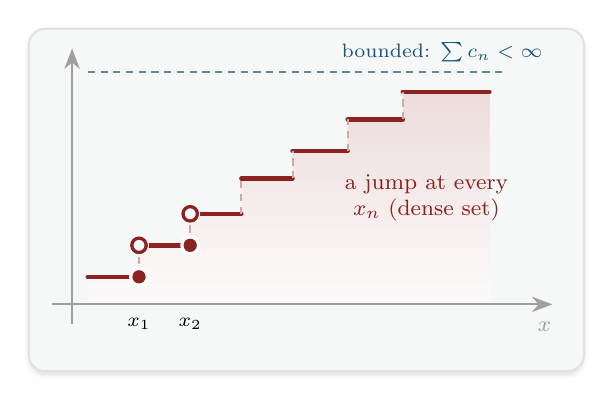
\begin{tikzpicture}[scale=1.0]
    \draw[panel] (-0.55,-0.85) rectangle (6.5,3.5);
    % area under the staircase
    \shade[top color=thmcolor!16, bottom color=thmcolor!2]
      (0.2,0.35) -- (0.85,0.35) -- (0.85,0.75) -- (1.5,0.75) -- (1.5,1.15)
      -- (2.15,1.15) -- (2.15,1.6) -- (2.8,1.6) -- (2.8,1.95) -- (3.5,1.95)
      -- (3.5,2.35) -- (4.2,2.35) -- (4.2,2.7) -- (5.3,2.7) -- (5.3,0) -- (0.2,0) -- cycle;
    % dashed bounded envelope (sum c_n converges -> bounded)
    \draw[projln, defcolor!70] (0.2,2.95) -- (5.5,2.95);
    \node[defcolor,font=\scriptsize,left] at (0.15,2.95) {};
    \node[defcolor,font=\scriptsize] at (4.7,3.2) {bounded: $\sum c_n<\infty$};
    % axes
    \draw[axisln] (-0.25,0) -- (6.1,0); \node[gray!75,font=\footnotesize] at (6.0,-0.28){$x$};
    \draw[axisln] (0,-0.25) -- (0,3.25);
    % monotone step function treads
    \def\steps{0.2/0.85/0.35, 0.85/1.5/0.75, 1.5/2.15/1.15, 2.15/2.8/1.6,
               2.8/3.5/1.95, 3.5/4.2/2.35, 4.2/5.3/2.7}
    \foreach \xs/\xe/\h in \steps {
      \draw[curveln,thmcolor] (\xs,\h) -- (\xe,\h);
    }
    % faint risers (the jumps)
    \foreach \xr/\hl/\hh in {0.85/0.35/0.75, 1.5/0.75/1.15, 2.15/1.15/1.6,
        2.8/1.6/1.95, 3.5/1.95/2.35, 4.2/2.35/2.7} {
      \draw[projln,thmcolor!40] (\xr,\hl) -- (\xr,\hh);
    }
    % highlight first two jumps with open/closed dots
    \opendot{thmcolor}{(0.85,0.75)} \dotpt{thmcolor}{(0.85,0.35)}
    \opendot{thmcolor}{(1.5,1.15)} \dotpt{thmcolor}{(1.5,0.75)}
    \node[below,font=\scriptsize] at (0.85,-0.05) {$x_1$};
    \node[below,font=\scriptsize] at (1.5,-0.05) {$x_2$};
    \node[thmcolor,font=\footnotesize,align=center] at (4.5,1.35)
      {a jump at every\\$x_n$ (dense set)};
  \end{tikzpicture}
  \end{center}

  \note{
    This sketch suggests what such a function looks like: a rising red
    staircase, with the shaded region beneath it, that takes a jump at every
    point of the dense set "E". The first two jumps, at "x" one and "x" two,
    are drawn with a solid dot at the lower level and an open dot just above, a
    reminder that this function is continuous from the left. Between the jumps
    the function is flat, and it is continuous there. Notice the blue dashed
    line near the top: because the weights "c" sub "n" sum to a finite total,
    all these infinitely many jumps together stay under that ceiling, giving a
    bounded, well defined increasing function. It is a striking object:
    discontinuous on a dense set, yet still monotonic and still subject to our
    countability theorem. The book notes that functions of this kind also arise
    later, in Theorem 6.16.
  }
\end{frame}

}

% =====================================================================
{
\usebackgroundtemplate{%
  
\includegraphics[width=\paperwidth,height=\paperheight,keepaspectratio=false]{chapter_04_bg_06.png}%
}
\section{Summary}
% =====================================================================

% --- Build 1/3 ---
\begin{frame}{Summary}
  \begin{hlbox}
  \textbf{Key takeaways:}
  \begin{itemize}
    \item \alert{Def 4.28:} monotonic = never decreasing or never increasing
  \end{itemize}
  \end{hlbox}

  \note{
    Let's review. We began with Definition 4.28: a function is monotonic if it
    either never decreases or never increases across the interval. This is the
    one structural assumption that drove everything else.
  }
\end{frame}

% --- Build 2/3 ---
\begin{frame}{Summary}
  \begin{hlbox}
  \textbf{Key takeaways:}
  \begin{itemize}
    \item \alert{Def 4.28:} monotonic = never decreasing or never increasing
    \item \alert{Thm 4.29:} both one-sided limits exist (sup / inf); no
      second-kind discontinuities
  \end{itemize}
  \end{hlbox}

  \note{
    Theorem 4.29 was the engine: for a monotonic function both one-sided limits
    exist at every point, given explicitly as a supremum on the left and an
    infimum on the right. An immediate corollary is that monotonic functions
    have no discontinuities of the second kind; every discontinuity is a simple
    jump.
  }
\end{frame}

% --- Build 3/3 ---
\begin{frame}{Summary}
  \begin{hlbox}
  \textbf{Key takeaways:}
  \begin{itemize}
    \item \alert{Def 4.28:} monotonic = never decreasing or never increasing
    \item \alert{Thm 4.29:} both one-sided limits exist (sup / inf); no
      second-kind discontinuities
    \item \alert{Thm 4.30:} discontinuities are at most countable --- but
      (4.31) can be dense
  \end{itemize}

  \vspace{0.5em}
  \textbf{Coming up next:} Infinite Limits and Limits at Infinity.
  \end{hlbox}

  \note{
    Theorem 4.30 then counted those jumps: there can be at most countably many,
    proved by tucking a distinct rational into each jump. And Remark 4.31
    showed the result is sharp, since the discontinuities can be dense. Next we
    turn to infinite limits and limits at infinity, extending our notion of
    limit to cover unbounded behavior and points at infinity. Thanks for
    watching, and see you in the next section.
  }
\end{frame}
}

\end{document}
